\section{Experiments}

\subsection{Datasets and Setup}

We evaluate our methods on the provided paired video super-resolution validation set. The low-resolution inputs are bicubic-downsampled sequences with scale factor $\times 4$, and the corresponding high-resolution frames are used as ground truth for quantitative evaluation. The validation inputs are stored in \texttt{val\_sharp\_bicubic/X4}, while the ground-truth frames are stored in \texttt{val\_sharp}. We report full-validation PSNR/SSIM results on all 30 validation sequences, containing 3000 frames in total. For detailed Direction C analysis, we additionally use validation sequences 000--006.

In addition to the paired validation set, we run qualitative inference on \texttt{REDS-sample}, \texttt{vimeo-RL}, and several custom videos such as \texttt{3.mp4}, \texttt{4.mp4}, \texttt{wild\_01}, and \texttt{wild\_05}. The \texttt{REDS-sample} and \texttt{vimeo-RL} folders in our workspace do not contain paired ground-truth frames, so they are used only for qualitative video outputs rather than PSNR/SSIM evaluation. We preserve the original folder structure when exporting videos. Specifically, we generate outputs for 10 REDS-sample sequences and 265 vimeo-RL sequences for both BasicVSR++ and Real-ESRGAN.

BasicVSR++ experiments are run in the MMagic environment, while Real-ESRGAN and the Part 3 hybrid pipeline are run in our Python virtual environment. All major experiments are conducted on a laptop GPU with 8GB VRAM. For large videos, we use chunked BasicVSR++ inference, tiled Real-ESRGAN inference when needed, and direct video writing to reduce memory and disk usage. For Part 2, we compare our fine-tuned BasicVSR++ checkpoint with our conservative fine-tuned Real-ESRGAN checkpoint on the full validation set.

\subsection{Metrics}

We use PSNR and SSIM as the main distortion metrics. PSNR measures pixel-level reconstruction fidelity, while SSIM measures structural similarity between the restored frame and the ground truth. These metrics are computed only on datasets with paired high-resolution ground truth, namely the provided validation set. For \texttt{REDS-sample}, \texttt{vimeo-RL}, and custom videos without ground truth, we provide qualitative videos and visual comparisons instead of PSNR/SSIM.

However, PSNR and SSIM do not fully capture perceptual sharpness or temporal stability. Therefore, for selected Part 3 experiments, we also report LPIPS and a simplified tLPIPS-style temporal proxy. LPIPS measures perceptual distance in a learned feature space. The temporal proxy measures perceptual changes between adjacent frames and is used as an approximate indicator of flickering. Since our temporal metric does not use optical-flow warping, we report it as a proxy rather than a full official tLPIPS implementation.

\subsection{Part 1 Baseline Results}

Table~\ref{tab:part1_results} reports the full validation results of the Part 1 baselines. SRCNN improves over bicubic and Lanczos interpolation, showing that a learned image super-resolution model can recover more structure than fixed interpolation. However, the simple temporal baseline performs worse because naive temporal aggregation can blur misaligned regions without explicit motion compensation.

\begin{table}[t]
\centering
\caption{Part 1 full-validation results. The temporal baseline uses neighboring-frame aggregation without explicit motion alignment.}
\label{tab:part1_results}
\resizebox{\linewidth}{!}{
\begin{tabular}{lccc}
\toprule
Method & Frames & PSNR & SSIM \\
\midrule
Bicubic & 3000 & 26.2949 & 0.7233 \\
Lanczos & 3000 & 26.5041 & 0.7302 \\
SRCNN & 3000 & 27.3264 & 0.7655 \\
Temporal Avg. w/o Align. & 3000 & 23.1046 & 0.6403 \\
\bottomrule
\end{tabular}
}
\end{table}

Figure~\ref{fig:part1_baseline} shows qualitative examples. Interpolation methods are smooth, SRCNN recovers slightly sharper structures, and the temporal baseline can blur details when motion is not aligned.

\begin{figure}[t]
\centering
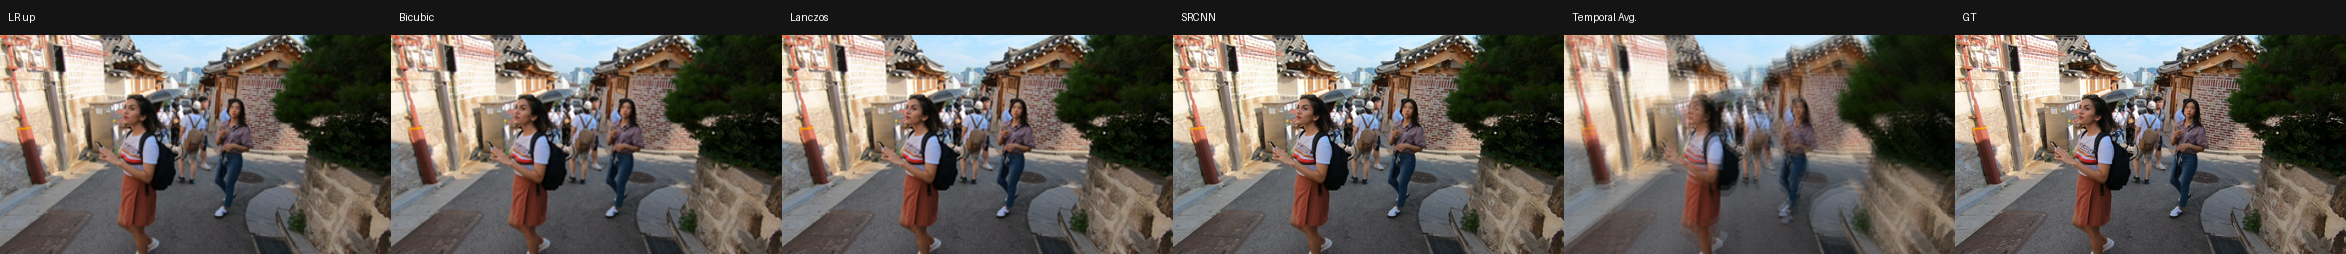
\includegraphics[width=\linewidth]{figures/part1_baseline_comparison.png}
\caption{Part 1 baseline comparison. Bicubic and Lanczos are smooth, SRCNN improves local structure, and the simple temporal baseline can blur misaligned details because it does not use motion alignment.}
\label{fig:part1_baseline}
\end{figure}

\subsection{Part 2 Model Comparison}

In Part 2, we evaluate BasicVSR++ and Real-ESRGAN as two complementary restoration branches. BasicVSR++ is more faithful and temporally stable because it uses information across frames. In contrast, Real-ESRGAN produces sharper local details but may hallucinate textures and reduce pixel-level fidelity. This difference makes BasicVSR++ suitable as the reliable reconstruction branch, while Real-ESRGAN is better viewed as a perceptual enhancement branch.

Table~\ref{tab:part2_full_val} reports the full-validation results of our fine-tuned BasicVSR++ and conservative fine-tuned Real-ESRGAN models. The validation set contains 30 sequences and 3000 frames. Fine-tuned BasicVSR++ achieves substantially higher PSNR and SSIM, confirming that the temporal model is more reliable for faithful reconstruction on the provided validation distribution. Fine-tuned Real-ESRGAN obtains lower distortion metrics, but it often produces sharper local edges and textures in qualitative examples.

\begin{table}[t]
\centering
\caption{Part 2 full-validation comparison between fine-tuned BasicVSR++ and conservative fine-tuned Real-ESRGAN.}
\label{tab:part2_full_val}
\resizebox{\linewidth}{!}{
\begin{tabular}{lccc}
\toprule
Model & Frames & PSNR & SSIM \\
\midrule
Fine-tuned BasicVSR++ & 3000 & 31.0021 & 0.8730 \\
Fine-tuned Real-ESRGAN & 3000 & 27.9661 & 0.7854 \\
\bottomrule
\end{tabular}
}
\end{table}

We also run both models on the unpaired \texttt{REDS-sample} and \texttt{vimeo-RL} folders for qualitative inspection. Since these folders do not include ground-truth frames in our workspace, they are not included in Table~\ref{tab:part2_full_val}. Instead, their outputs are saved as videos while preserving the original data structure. This provides additional visual evidence on out-of-validation inputs without mixing unpaired data into the quantitative evaluation.

Figure~\ref{fig:part2_compare} compares the two fine-tuned Part 2 models on a representative validation frame. BasicVSR++ better preserves structure and temporal fidelity, while Real-ESRGAN tends to sharpen local details more aggressively. This supports the motivation for the Part 3 hybrid system: Real-ESRGAN should not globally replace BasicVSR++, but it can still be useful when applied selectively.

\begin{figure}[t]
\centering
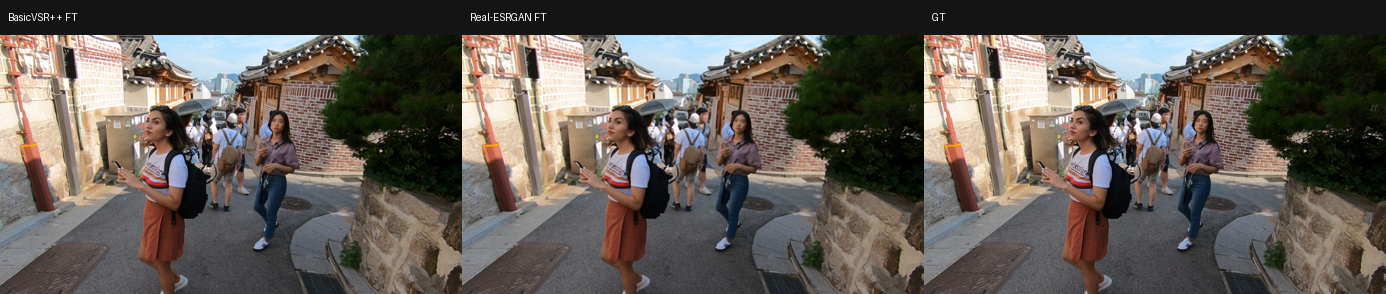
\includegraphics[width=\linewidth]{figures/part2_basicvsrpp_vs_realesrgan_finetuned.png}
\caption{Part 2 qualitative comparison using fine-tuned models. Fine-tuned BasicVSR++ preserves structure and temporal fidelity, while fine-tuned Real-ESRGAN produces sharper but less faithful perceptual details.}
\label{fig:part2_compare}
\end{figure}

\subsection{Part 3 Direction C Results}

Table~\ref{tab:directionc_val000} reports the main Direction C comparison on validation sequence 000. Standalone Real-ESRGAN performs much worse than BasicVSR++ in PSNR, SSIM, LPIPS, and the temporal proxy, indicating that unrestricted generative enhancement introduces artifacts and unstable details. The Direction C hybrid stays close to BasicVSR++ across all metrics, showing that the alpha mask successfully limits the generative branch.

\begin{table}[t]
\centering
\caption{Direction C results on validation sequence 000. Lower is better for LPIPS and tLPIPS proxy.}
\label{tab:directionc_val000}
\resizebox{\linewidth}{!}{
\begin{tabular}{lcccc}
\toprule
Method & PSNR & SSIM & LPIPS$\downarrow$ & tLPIPS-p$\downarrow$ \\
\midrule
BasicVSR++ & 31.4585 & 0.8871 & 0.1590 & 0.1541 \\
Official Real-ESRGAN & 24.1239 & 0.6656 & 0.2537 & 0.2477 \\
Direction C Hybrid & 31.3772 & 0.8860 & 0.1610 & 0.1565 \\
\bottomrule
\end{tabular}
}
\end{table}

Figure~\ref{fig:part3_mask} visualizes the hybrid result and the alpha mask. The mask is conservative in reliable structural regions and allows more generative contribution in uncertain texture regions.

\begin{figure}[t]
\centering
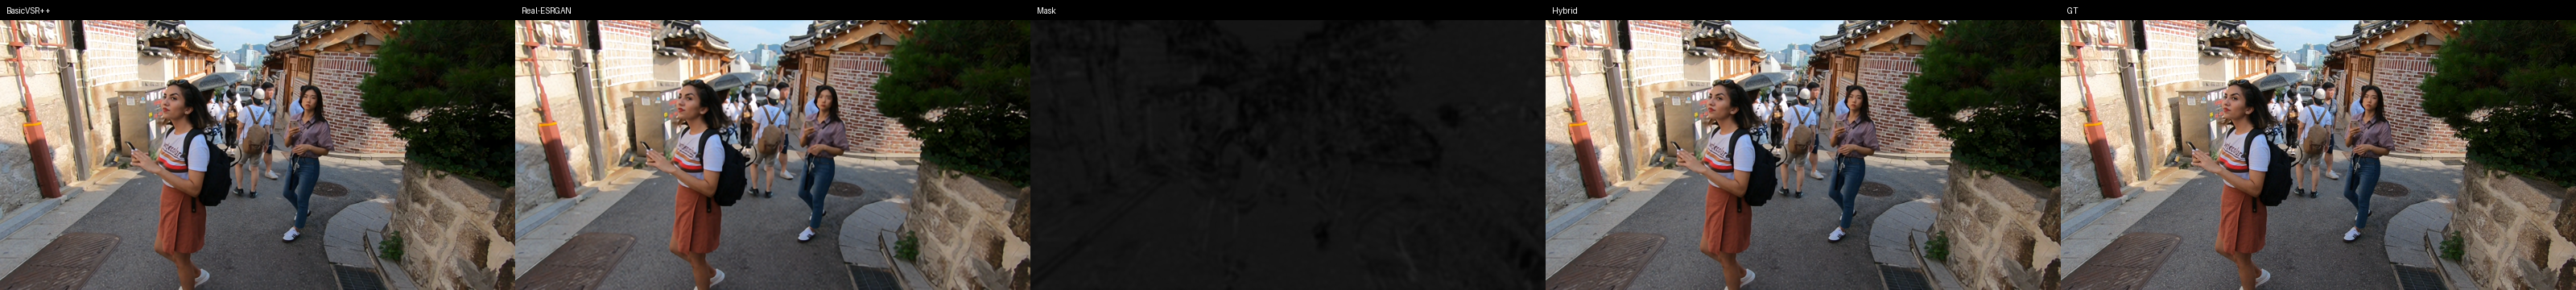
\includegraphics[width=\linewidth]{figures/part3_mask_basic_real_hybrid.png}
\caption{Part 3 Direction C visualization. The hybrid output uses BasicVSR++ as the reliable reconstruction branch and selectively introduces Real-ESRGAN details through the adaptive alpha mask.}
\label{fig:part3_mask}
\end{figure}

We further evaluate two Direction C parameter variants on validation sequences 000--006. The conservative variant uses a lower Real-ESRGAN contribution and is selected as our formal result. The anime-stronger variant increases the alpha value and weakens structure protection, making the output sharper but less faithful to the ground truth.

\begin{table}[t]
\centering
\caption{Direction C parameter ablation on validation sequences 000--006.}
\label{tab:directionc_ablation}
\resizebox{\linewidth}{!}{
\begin{tabular}{lcccc}
\toprule
Variant & Frames & PSNR & SSIM & Mean $\alpha$ \\
\midrule
Conservative & 700 & 32.8052 & 0.9075 & 0.11--0.15 \\
Anime-stronger & 700 & 32.1390 & 0.8934 & 0.29--0.32 \\
\bottomrule
\end{tabular}
}
\end{table}

The ablation confirms the perception-fidelity trade-off. Increasing the Real-ESRGAN contribution can improve subjective sharpness, especially on anime-style content, but it reduces PSNR and SSIM on the validation set. Therefore, we use the conservative variant as the main Direction C result.

\subsection{Qualitative Analysis}

Figure~\ref{fig:directionc_showcase} shows the full Direction C diagnostic visualization. The showcase includes BasicVSR++, Real-ESRGAN, the final hybrid output, the alpha mask, structure protection, uncertain texture, hallucination risk, and flicker risk. These maps make the decision process interpretable. Regions with high hallucination or flicker risk are suppressed, while uncertain texture regions can receive limited generative enhancement.

\begin{figure*}[t]
\centering
\includegraphics[width=\textwidth]{part3/results/adaptive_hybrid_000_directionc_official/showcase_00000049.png}
\caption{Full Direction C showcase. The diagnostic maps explain how the hybrid method protects reliable structures and selectively introduces Real-ESRGAN details in uncertain texture regions.}
\label{fig:directionc_showcase}
\end{figure*}

On custom anime-style videos, we observe that pure Real-ESRGAN can sometimes look sharper than the conservative hybrid. This is expected because anime content has clean edges and flat color regions that match Real-ESRGAN's strengths. However, for real-world videos, the conservative hybrid is more reliable because it avoids applying generative enhancement globally. This supports our main interpretation: Direction C is not designed to produce the sharpest possible frame in every case, but to control hallucination and flicker risks while preserving the stability of BasicVSR++.
